\documentclass{beamer}

\usepackage{tikz}
\usepackage{pgfplots}
\usepackage{fontawesome5}
\pgfplotsset{compat=1.18}
\usepackage[UTF8]{ctex}
\usepackage[T1]{fontenc}
\usepackage{beamerthemesplit}
\usefonttheme[onlymath]{serif}
\usetheme{Warsaw}

\usepackage{listings}
\usepackage{xcolor}

% 定义漂亮的 C++ 代码高亮风格
\lstset{
	language=C++,
	basicstyle=\ttfamily\footnotesize,       % 基本字体和大小
	keywordstyle=\color{blue}\bfseries,      % 关键字颜色：蓝色加粗
	commentstyle=\color{green!50!black}\itshape, % 注释颜色：深绿色斜体
	stringstyle=\color{red},                 % 字符串颜色：红色
	showstringspaces=false,                  % 不显示字符串中的空格标记
	numbers=left,                            % 左侧显示行号
	numberstyle=\tiny\color{gray},           % 行号字体设置
	stepnumber=1,                            % 每 1 行显示一次行号
	breaklines=true,                         % 自动换行
	frame=single,                            % 给代码加个边框 (也可以用 lines)
	backgroundcolor=\color{black!5},         % 浅灰色背景
	morekeywords={pragma, omp, parallel, schedule, static}, % 让 OpenMP 指令也能高亮
	escapechar=|                             % 允许在代码中使用 |...| 插入 LaTeX 命令（用于特殊标记）
}

\title[]{SpMV 算法的多核并行性能基准测试}
\author[Peruere1828（南京大学）]{汇报人：Peruere1828}
\institute[南京大学]{南京大学，\\
		fmyh1828@gmail.com}
\date{\today}

\bibliographystyle{plain}
\setbeamertemplate{bibliography item}[text]

\begin{document}
	
	\begin{frame}
		\titlepage
	\end{frame}

	\begin{frame}{什么是 SpMV？}
	\begin{equation*}
		\mathbf{y} = A \mathbf{x}
	\end{equation*}
	\begin{itemize}
		\item $A$: 稀疏矩阵
		\item $\mathbf{x}, \mathbf{y}$: 稠密向量
	\end{itemize}
	
	\vskip 0.5cm
	\begin{itemize}
		\item \textbf{应用场景}：科学计算、图像处理、AI图神经网络、流体力学模拟的核心底层。
	\end{itemize}
\end{frame}
	
	\begin{frame}{什么是稀疏矩阵？}
		\textbf{定义}：矩阵中\textbf{绝大多数元素都是 0} 的矩阵。
		
		\textbf{生活中的例子}：
		\begin{itemize}
			\item \textbf{社交网络}：全球有数十亿用户（对应行与列），但每个人通常只认识几百人。如果我们用“1”表示认识、“0”表示不认识，那么整个社交关系矩阵就会非常庞大，且绝大多数位置都是0——这就是一个典型的稀疏矩阵。
		\end{itemize}
		
		如果强行存下所有0，会导致大量的\textbf{内存浪费}和\textbf{无效计算}。
	\end{frame}
	
	\begin{frame}{稀疏矩阵的存储：CSR格式}
		设稀疏矩阵 $A \in \mathbb{R}^{N \times M}$ 共有 $NNZ$ 个非零元。CSR 格式将其压缩为三个一维数组：
		\vskip 0.3cm
		
		\begin{columns}
			% 左侧：数学化定义
			\begin{column}{0.5\textwidth}
				\begin{itemize}
					\item \textbf{数值数组} $\mathbf{V} \in \mathbb{R}^{NNZ}$ \\
					\small 依次存储所有 $A_{i,j} \neq 0$ 的实际值。
					
					\vskip 0.2cm
					\item \textbf{列索引数组} $\mathbf{C} \in \mathbb{Z}^{NNZ}$ \\
					\small $\mathbf{C}[k] = j$，记录 $\mathbf{V}[k]$ 所在的列号。
					
					\vskip 0.2cm
					\item \textbf{行指针数组} $\mathbf{R} \in \mathbb{Z}^{N+1}$ \\
					\small $\mathbf{R}[i]$ 指向第 $i$ 行在 $\mathbf{V}$ 和 $\mathbf{C}$ 中的起始下标。\\
					\textcolor{blue}{第 $i$ 行的非零元数量 $\Delta = \mathbf{R}[i+1] - \mathbf{R}[i]$}。
				\end{itemize}
			\end{column}
			
			% 右侧：你的图片
			\begin{column}{0.48\textwidth}
				\centering
				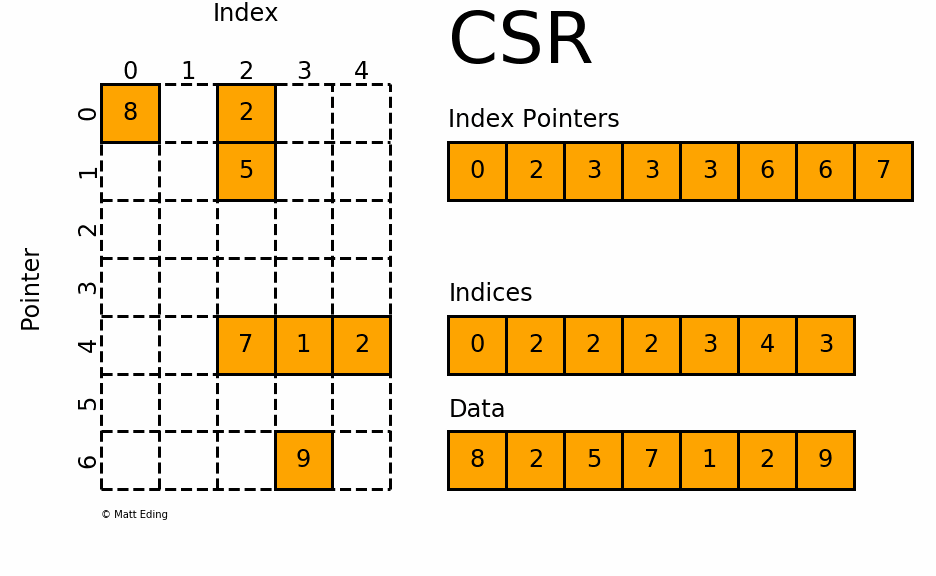
\includegraphics[width=\textwidth]{CSR.png}
			\end{column}
		\end{columns}
		
	\end{frame}
	
%	\section{MLIR Pass Pipeline 自动生成探索}

\begin{frame}[fragile]{核心代码：基于 CSR 的 OpenMP 并行 SpMV}
	
	\begin{block}{标准的 CSR-SpMV 并行实现}
		\vspace{-0.2cm} % 稍微上移一点，显得更紧凑
		\begin{lstlisting}
void spmv_omp(const CSR &A, const float *x, float *y) {
  const int *rp = A.row_ptr;
  const int *ci = A.col_idx;
  const float *vl = A.val;
  
#pragma omp parallel for schedule(static)
  for (int i = 0; i < A.n; i++) {
    float sum = 0.0f;
    for (int j = rp[i]; j < rp[i + 1]; j++) {
      // |\color{red}\textbf{间接寻址：通过 ci[j] 访问稠密向量 x}|
      sum += vl[j] * x[ci[j]]; 
    }
    y[i] = sum;
  }
}
		\end{lstlisting}
	\end{block}
\end{frame}

\begin{frame}[fragile]{对比基准：开源库 Eigen 的实现}
	\begin{block}{Eigen 稀疏矩阵向量乘法核心逻辑}
		\vspace{-0.1cm}
		\begin{lstlisting}
Eigen::SparseMatrix<float, Eigen::RowMajor> Em(N, M);

// |\color{red}\textbf{将 CSR 格式的稀疏矩阵 A 填入 Em}|
vector<Eigen::Triplet<float>> trips;
for (int i = 0; i < N; i++)
  for (int j = A.row_ptr[i]; j < A.row_ptr[i+1]; j++)
    trips.emplace_back(i, A.col_idx[j], A.val[j]);
Em.setFromTriplets(trips.begin(), trips.end());

// |\color{red}\textbf{将稠密向量 x 映射到 ex}|
Eigen::Map<Eigen::VectorXf> ex(x, M);
Eigen::VectorXf ey(N);

ey = Em * ex;
		\end{lstlisting}
	\end{block}
\end{frame}

\begin{frame}{实验设计：测试环境与矩阵数据集}
	\begin{itemize}
		\item \textbf{硬件平台}：南大集群 7702ib 队列，单节点 20 核心
		\item \textbf{编译环境}：GCC 11.2.0 (\texttt{-O3 -march=native}) + OpenMP 并行
		\item \textbf{对比库}：Eigen 3.4.0 (业界知名 C++ 矩阵库)
		\item \textbf{测试数据}：来自 SuiteSparse 矩阵集（工业界真实问题）
	\end{itemize}
	
	\vskip 0.3cm
	\begin{table}
		\small
		\centering
		\begin{tabular}{l|l|r|r}
			\hline
			\textbf{矩阵名称} & \textbf{来源领域} & \textbf{大小 (N)} & \textbf{非零元 (NNZ)} \\ \hline
			parabolic\_fem & 流体力学问题 & 525,825 & 3.67 M \\
			apache2 & 结构力学问题 & 715,176 & 4.81 M \\
			pre2 & 电路仿真模拟 & 659,033 & 5.95 M \\
			amazon0312 & 亚马逊网络有向图 & 400,727 & 3.20 M \\
			neos3 & 线性规划问题 & 512,209 & 2.05 M \\
			wheel\_601 & 组合数学问题 & 902,103 & 2.17 M \\ \hline
		\end{tabular}
	\end{table}
\end{frame}

\begin{frame}{性能结果：在真实矩阵上的加速 (20 Threads)}
	\centering
	\begin{tikzpicture}
		\begin{axis}[
			ybar,
			width=0.9\textwidth,
			height=0.7\textheight,
			ylabel={Speedup vs. Serial CSR},
			ymin=0,
			bar width=8pt,
			enlarge x limits=0.2,
			symbolic x coords={parabolic\_fem, apache2, pre2, amazon0312, neos3, wheel\_601},
			xtick=data,
			x tick label style={rotate=30, anchor=east, font=\footnotesize},
			nodes near coords,
			point meta=explicit symbolic,
			every node near coord/.append style={font=\tiny, anchor=west, rotate=90, xshift=2pt},
			legend style={at={(0.5,-0.3)}, anchor=north, legend columns=-1},
			title={OpenMP vs. Eigen SpMV Performance}
			]
			\addplot[fill=blue!40] coordinates {
				(parabolic\_fem, 8.8)
				(apache2, 8.3)
				(pre2, 9.0)
				(amazon0312, 10.2)
				(neos3, 9.4)
				(wheel\_601, 17.4)
			};
			\addplot[fill=red!40] coordinates {
				(parabolic\_fem, 2.1)
				(apache2, 1.7)
				(pre2, 1.9)
				(amazon0312, 4.4)
				(neos3, 4.1)
				(wheel\_601, 6.2)
			};
			\legend{OpenMP, Eigen}
		\end{axis}
	\end{tikzpicture}
\end{frame}
	
\begin{frame}{性能结果：OpenMP 多线程加速表现}
	\begin{itemize}
		\item 评估指标：\textbf{GFLOPS}（每秒十亿次浮点运算，越高越好）
	\end{itemize}
	
	\vskip 0.2cm
	\begin{columns}
		\begin{column}{0.55\textwidth}
			% 使用 pgfplots 绘制折线图
			\begin{tikzpicture}
				\begin{axis}[
					width=\textwidth,
					height=5.5cm,
					title={使用parabolic\_fem矩阵},
					xlabel={线程数 (Threads)},
					ylabel={性能 (GFLOPS)},
					xmin=0, xmax=22,
					ymin=0, ymax=25,
					xtick={1, 2, 4, 8, 16, 20},
					ymajorgrids=true,
					grid style=dashed,
					legend pos=north west,
					label style={font=\footnotesize},
					tick label style={font=\footnotesize}
					]
					\addplot[
					color=red,
					mark=square*,
					line width=1.2pt
					] coordinates {
						(1, 2.30)
						(2, 3.49)
						(4, 5.73)
						(8, 12.08)
						(16, 14.88)
						(20, 20.26)
					};
					\addlegendentry{\scriptsize 实际测算性能}
				\end{axis}
			\end{tikzpicture}
		\end{column}
		
		\begin{column}{0.45\textwidth}
			\begin{block}{现象分析}
				\small
				\textbf{未能实现线性加速：}\\
				在 20 线程满载时，性能达到 \textbf{20.26 GFLOPS}（约 8.8 倍加速）。\\
				\vskip 0.2cm
				\textbf{原因（访存受限）：}\\
				随着线程数增加，总内存带宽逐渐饱和。多核同时抢占内存总线，导致加速效率递减。
			\end{block}
		\end{column}
	\end{columns}
\end{frame}

\begin{frame}{拓展探究：换个视角看矩阵 —— CSC 格式}
	除了按行压缩的 CSR，工业界（如 Eigen 默认设置）还常用\textbf{按列压缩的 CSC 格式}。
	\vskip 0.3cm
	
	\begin{columns}
		\begin{column}{0.48\textwidth}
			\begin{block}{CSR (按行计算)}
				\small
				每一行计算一个唯一的 \texttt{y[i]}。\\
				读取多个 \texttt{x}，累加后\textbf{一次性安全写入} \texttt{y[i]}。\\
				不同线程算不同的行，互不干扰。
			\end{block}
		\end{column}
		
		\begin{column}{0.48\textwidth}
			\begin{block}{CSC (按列计算)}
				\small
				每一列只读取一个 \texttt{x[j]}。\\
				但要把结果\textbf{分散累加}到多个不同的 \texttt{y} 元素中。\\
				不同线程可能同时修改同一个 \texttt{y}。
			\end{block}
		\end{column}
	\end{columns}
	
	\vskip 0.4cm
	
	CSC 格式中，由于多个线程可能同时修改同一个 \texttt{y[i]}，所以必须使用原子操作。
\end{frame}

\begin{frame}[fragile]{核心代码：基于 CSC 的 OpenMP 并行 SpMV}
	
	\begin{block}{标准的 CSC-SpMV 并行实现}
		\vspace{-0.2cm} % 稍微上移一点，显得更紧凑
		\begin{lstlisting}
void spmv_csc(const CSC &A, const float *x, float *y) {
  const int *cp = A.col_ptr;
  const int *ri = A.row_idx;
  const float *vl = A.val;
  const int N = A.n, M = A.m;
  memset(y, 0, N * sizeof(float));
  
#pragma omp parallel for schedule(static)
  for (int j = 0; j < M; j++) {
    float xj = x[j];
    for (int k = cp[j]; k < cp[j + 1]; k++) {
#pragma omp atomic
      y[ri[k]] += vl[k] * xj;
    }
  }
}
		\end{lstlisting}
	\end{block}
\end{frame}

\begin{frame}{性能结果：在真实矩阵上的加速 (20 Threads)}
	\centering
	\begin{tikzpicture}
		\begin{axis}[
			ybar,
			width=0.9\textwidth,
			height=0.7\textheight,
			ylabel={Speedup vs. CSR},
			ymin=0,
			bar width=8pt,
			enlarge x limits=0.2,
			symbolic x coords={parabolic\_fem, apache2, pre2, amazon0312, neos3, wheel\_601},
			xtick=data,
			x tick label style={rotate=30, anchor=east, font=\footnotesize},
			nodes near coords,
			point meta=explicit symbolic,
			every node near coord/.append style={font=\tiny, anchor=west, rotate=90, xshift=2pt},
			legend style={at={(0.5,-0.3)}, anchor=north, legend columns=-1},
			title={CSR vs. CSC Performance}
			]
			\addplot[fill=blue!40] coordinates {
				(parabolic\_fem, 15.83)
				(apache2, 15.63)
				(pre2, 14.91)
				(amazon0312, 12.27)
				(neos3, 11.25)
				(wheel\_601, 11.22)
			};
			\addplot[fill=red!40] coordinates {
				(parabolic\_fem, 1.97)
				(apache2, 3.42)
				(pre2, 2.67)
				(amazon0312, 0.86)
				(neos3, 0.38)
				(wheel\_601, 0.88)
			};
			\addplot[fill=green!40] coordinates {
				(parabolic\_fem, 1.67)
				(apache2, 1.52)
				(pre2, 1.66)
				(amazon0312, 0.95)
				(neos3, 1.69)
				(wheel\_601, 1.24)
			};
			\legend{CSR, CSC, CSC\_serial}
		\end{axis}
	\end{tikzpicture}
\end{frame}

\begin{frame}{为什么 CSC 表现如此糟糕？}
	\begin{block}{}
		\begin{itemize}
			\item \textbf{CSR 零竞争}：按行分拆，每线程独立写自己的 \texttt{y[i]}，互不干扰。
			\item \textbf{CSC 写冲突}：无论使用 Buffer 归约还是 \texttt{atomic} 原子加，\textbf{都无法避免多核抢夺并覆写同一行的数据。} 这是格式决定的物理限制。
		\end{itemize}
	\end{block}
	
	\vskip 0.3cm
	
	\textbf{为什么在 \texttt{neos3} 和 \texttt{wheel\_601} 上尤其糟糕}：
	\begin{itemize}
		\item 这类矩阵平均每列仅 \textbf{2$\sim$4} 个非零元，且非零元高度集中在少数几个核心行上。
		\item \textbf{后果}：20 个核心的算力没有转化为吞吐量，反而全部堵在争夺那几行的原子锁上，导致许多额外开销。
	\end{itemize}

\end{frame}

\begin{frame}{更多话题……}
	\begin{itemize}
		\item CSC 在 SpMV 上表现糟糕，但是适合其它需要按列分析矩阵的问题。
		\item 如何把各种稀疏矩阵格式转来转去？更高维的稀疏张量呢？
		\item 在 GPU 上怎么实现 SpMV？
	\end{itemize}
	
\vfill

\begin{block}{参考资源 \& 推荐阅读}
	\footnotesize
	\begin{itemize}
		\item [\faLink] \textbf{稀疏格式描述与转换}：\href{https://mlir.llvm.org/docs/Dialects/SparseTensorOps/}{MLIR sparse\_tensor Dialect}（用统一的仿射抽象来描述各类稀疏格式）
		\item [\faLink] \textbf{GPU 上的 SpMV}：\href{https://developer.nvidia.com/cusparse}{NVIDIA cuSPARSE Library Documentation}
		\item [\faLink] \textbf{数据集来源}：\href{https://sparse.tamu.edu/}{SuiteSparse Matrix Collection}
	\end{itemize}
\end{block}
\end{frame}

	\begin{frame}
		\begin{center}
			\Large{敬请各位批评指正！}
		\end{center}
	\end{frame}
	
\end{document}